\exercice{Étamage}
    \begin{figure}[!ht]
      \centering
      \begin{circuitikz}
  \draw[very thick]
    (-1,-3) -- (-1,0)
    (1,-3) -- (1,0)
  ;
  \draw
    (-2,0) -- (-2,-4) -- (2,-4) -- (2,0)
    (-2,-1) -- (2,-1)
  ;
  \draw
    (-1,0) -- (-1,1) to[V={$E{=}\SI{3}{V}$}] (1,1) -- (1,0);
\end{circuitikz}
  

    
  
    \end{figure}
    
    Une application importante de l'étain est l’étamage : une boite de conserve en fer blanc est formée d’une tôle d’acier recouverte d’une fine couche d’étain pour la protéger.
    
    Une expérience d’étamage est effectuée à la température de $\SI{25}{\celsius}$ sur un échantillon de fer de surface totale $S = \SI{240}{cm^2}$ . L’électrolyte est constitué d’acide 4-hydroxybenzènesulfonique et d’une solution d’ions $\ce{Sn^2+}$ ; différents produits d’addition maintiennent son $pH$ à une valeur proche de $0$. L’étain intervient pour cette étude par le couple rédox $\ce{Sn^2+ /Sn(s)}$.

    \begin{enumerate}
      \question{Le potentiel standard du couple $\ce{H+/H2(g)}$ n'est pas donné, pourquoi ?}
        [Quelle origine a été choisie pour les potentiels électriques en électrochimie ?]
      \question{Compléter le schéma de la figure, en précisant la polarité du générateur ainsi que le sens de passage du courant. Qualifier chaque électrode du terme << anode >> ou << cathode >>.}
        [Dans quel sens se déplacent les électrons ? Quelle réaction se produit à l'électrode où arrivent les électrons ? A celle d'où ils partent ?]
        [L'idée de l'étamage est de déposer de l'étain sur du fer. En déduire quelle électrode a quelle nature.]
    \end{enumerate}
   
    
    La surtension cathodique du couple $\ce{H+ (aq)/H2 (g)}$ ( $\eta_c = -\SI{0,40}{V}$) est la même sur le fer et sur l’étain. Le couple $\ce{Sn^2+ /Sn(s)}$ est rapide sur le fer et sur l’étain ; l’acide 4-hydroxybenzènesulfonique est considéré comme inerte.
    \begin{enumerate}
      \setcounter{enumi}{2}
      \question{Un petit dégagement gazeux est observé au niveau de l’électrode en fer. Quel est-il ?}
        [Quelle espèce présente dans la solution peut produire un gaz par oxydation et réduction ?]
        [La réaction a-t-elle lieu à l'anode ou à la cathode ? Est-ce une oxydation ou une réduction ? S'agit-il donc de la formation de $\ce{O2}$ ou $\ce{H2}$ ?]
      \question{Écrire les échanges électroniques au niveau de chaque électrode et représenter les courbes intensité-potentiel correspondant à ces échanges.}
        [Le fer réagit-il ?]
        [Représenter la courbe i-E de l'étain. Possède-t-elle des surpotentiels ? Un ou des paliers de saturation ?]
        [Tracer le mur du solvant en prenant en compte le surpotentiel indiqué.]
      \question{Exprimer puis calculer la masse $m$ d’étain maximale déposée sur le fer, sachant que l’intensité totale du courant est $i = \SI{1,0}{A}$ et que l’électrolyse est arrêtée au bout de $\SI{4}{min}$.}
        [Intégrer la relation entre courant électrique et vitesse de réaction.]
      \question{En réalité, la masse mesurée est $\SI{0.12}{g}$. Calculer le rendement Faradique.}
    \end{enumerate}

    \paragraph{Données} Masse molaire de l'étain : $M(\ce{Sn})=\SI{118.7}{g.mol^{-1}}$.
    \begin{table}[!h]
      \centering
      \begin{tabular}{|c|c|c|c|c|}
        \hline
        Couple & $\ce{Fe^2+/Fe(s)}$ & $\ce{Sn^2+/Sn(s)}$ & $\ce{H+/H2(g)}$ & $\ce{O2(g)/H2O(l)}$\\
        \hline
        $E^0 (V)$ & $\SI{-0.44}{}$ & $\SI{-0.14}{}$ &  & $\SI{1.23}{}$\\
        \hline
      \end{tabular}
    \end{table}
    

  \exercice{Étude du zinc}
    On étudie une solution contenant des ions $\ce{Zn^2+}$, accompagnés d’impuretés cationiques. On ne prendra en compte que les impuretés suivantes : $\ce{Cd^2+}$ , $\ce{Cu^2+}$ et $\ce{Ni^2+}$. On procède alors à un ajout de zinc solide (en poudre) dans la solution dans le but de purifier la solution.
    \begin{figure}[!ht]
      \centering
      
\includegraphics[width=.8\linewidth]{figures/2.png}
    \end{figure}
    \begin{enumerate}
      \question{À l’aide de la figure, justifier le procédé de purification en écrivant les équations bilans des différentes réactions qui ont lieu. Sous quelles formes sont alors les impuretés ? Comment peut-on les éliminer ?}
        [Quelle réaction se produira si on met en contact du zinc solide et une solution contenant des ions $\ce{Cd2+}$ ? Raisonner de même pour $\ce{Ni2+}$ et $\ce{Cu2+}$]
    \end{enumerate}

    On obtient une solution de sulfate de zinc à $\SI{2}{mol.L^{-1}}$ que l’on acidifie par de l’acide sulfurique à $\SI{1,5}{mol.L^{-1}}$. Les activités de $\ce{H+}$, $\ce{O2}$ et $\ce{H2}$ seront prises égales à $1$. Pour obtenir du zinc sous forme métallique solide, on procède à l’électrolyse de cette solution. Les électrodes utilisées sont : cathodes en aluminium et anodes en plomb inattaquables en milieu sulfate. Les cuves sont en ciment revêtues de polychlorure de vinyle (PVC).

    \begin{enumerate}
      \setcounter{enumi}{1}
      \question{Nous considérerons dans la suite que les ions sulfate ne participent à aucune réaction. D’un point de vue thermodynamique, quelles sont les réactions qui peuvent avoir lieu à la cathode ? À l’anode ? En déduire la réaction d’électrolyse attendue. Quelle différence de potentiel devrait-on appliquer ?}
        [Lister tous les réducteurs présents et les couples associés. Quelle(s) réaction(s) peuvent se produire à l'anode ? Même question pour la cathode.]
        [En comparant les potentiels de Nernst des différents couples, quelle réaction est la plus thermodynamiquement favorable (ou plutôt la moins défavorable puisqu'il s'agit d'une réaction forcée) ?]
      \question{À l’aide de la figure suivante, donner l’équation d’électrolyse qui a réellement lieu. À quoi sont dus ces changements ? Si on impose une densité de courant de \SI{500}{A.m^{-2}}, quelle devrait être la différence de potentiel appliquée aux bornes des électrodes ? Estimer approximativement le rendement faradique associé au dépôt de zinc à la cathode.}
        [Quelle réaction devient la plus facile à forcer ?]
        [Pourquoi la réaction $\ce{H+ -> H2}$ de démarre pas à $\SI{0}{V}$ ?]
        [Quel potentiel faut-il imposer à l'électrode d'aluminium pour que son courant TOTAL soit de $\SI{-500}{A}$ ?]
        [Quelle proportion du courant sert alors à la réaction voulue ?]
    \end{enumerate}
    
    \begin{figure}[!ht]
      \centering
      
\includegraphics[width=.8\linewidth]{figures/3.png}
    \end{figure}
      
  \exercice{Raffinage électrolytique du cuivre}
    Une lame de cuivre plonge dans une solution de nitrate d’argent. Les courbes intensité-potentiel relatives aux différents couples en présence sont représentées ci-dessous.
    \begin{figure}[!ht]
      \centering
      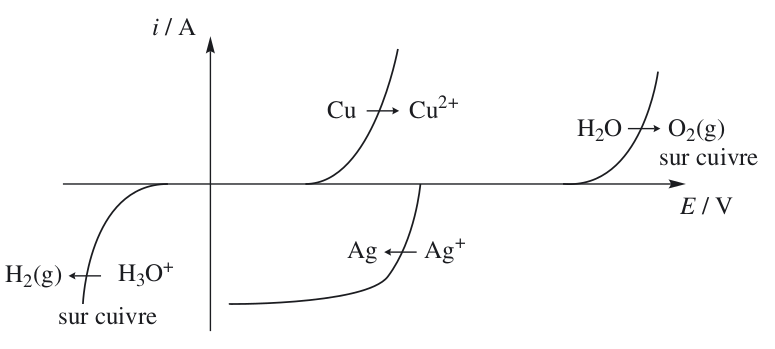
\includegraphics[width=.8\linewidth]{figures/4.png}
    \end{figure}
    
    \begin{table}[!h]
      \centering
      \begin{tabular}{|c|c|c|c|c|}
        \hline
        Couple & $\ce{Pb^2+/Pb(s)}$ & $\ce{Cu^2+/Cu(s)}$ & $\ce{Ag+/Ag(s)}$ & $\ce{O2(g)/H2O(l)}$\\
        \hline
        $E^0 (V)$ & $\SI{-0.13}{}$ & $\SI{0.34}{}$ & $\SI{0.80}{}$ & $\SI{1.23}{}$\\
        \hline
      \end{tabular}
      \caption*{Données}
    \end{table}
    \begin{enumerate}
      \question{Écrire l’équation-bilan de la réaction qui a lieu. Déterminer sa constante d’équilibre à $\SI{298}{K}$. Commenter la valeur obtenue.}
        [Faire une échelle de potentiel et mettre en évidence les espèces présentes. Quelle est la réaction la plus thermodynamiquement favorable ?]
        [Comment l'enthalpie libre standard de réaction est-elle reliée à la différence de potentiels standards ? À la constante de réaction ?]
        [Que peut-on dire quand $K^\circ\gg 1$ ?]
      \question{À l’aide des courbes intensité-potentiel, prévoir si cette réaction est rapide ou lente (un schéma est souhaité).}
        [Quel unique potentiel permet l'égalité de la somme des courants anodiques et la somme des courants cathodiques ? Ce potentiel permet-il un courant significatif ?]
    \end{enumerate}
    Le raffinage électrolytique du cuivre consiste à placer du cuivre impur comme anode dans une solution concentrée de sulfate de cuivre. Une électrode support (en acier inoxydable) est placée en vis-à-vis pour y déposer le cuivre par réduction cathodique. Les seules impuretés qui seront considérées ici sont le plomb $\ce{Pb}$ et l’argent $\ce{Ag}$. Le système est modélisé de façon simple par une électrode de cuivre comportant des particules d’argent pur et de plomb pur (cette modélisation est une approximation de la réalité : il existe probablement une solution solide de plomb/argent dans le cuivre). Les  courbes intensité-potentiel relatives aux différents couples en présence sont représentées ci-dessous. $E_A$ désigne le potentiel auquel est portée l’anode, et $E_C$ celui de la cathode.
    \begin{figure}[!ht]
      \centering
      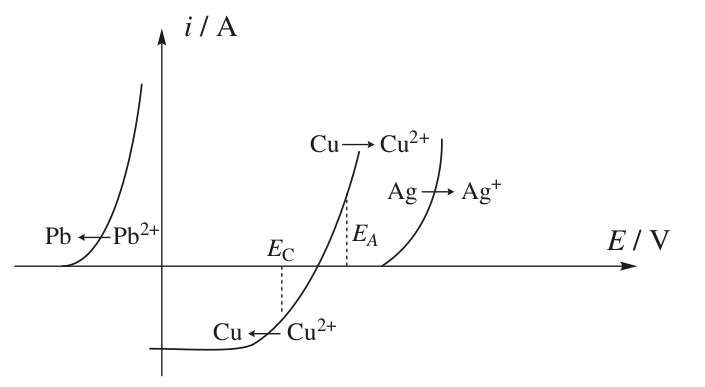
\includegraphics[width=.8\linewidth]{figures/5.png}
    \end{figure}
    \begin{enumerate}
      \setcounter{enumi}{2}
      \question{Écrire la(les) réaction(s) observée(s) à l’anode. Même question à la cathode.}
        [Le potentiel $E_A$ permet-il l'oxydation de $\ce{Pb}$ ? de $\ce{Cu}$ ? de $\ce{Ag}$ ?]
        [Parmi les solutés produits, lesquels peuvent être réduits au potentiel $E_C$ ?]
      \question{Expliquer l’intérêt de cette méthode quant à la purification du cuivre.}
        [Les impuretés présentes à l'anodes sont-elles reformées à la cathode ?]
    \end{enumerate}
    

  \exercice{Corrosion du zinc}
    On considère un litre d’eau désaérée par un barbotage de gaz argon (qui chasse $\ce{O2}$ dissous) à $pH = \SI{6.0}{}$ sous $p = p^0$ et $T = \SI{298}{K}$. Une tôle en acier électro-zingué est introduite (tôle recouverte de zinc solide). On admet que la concentration en ions zinc(II) est donnée par $\left[\ce{Zn^2+}\right]=\SI{1e-6}{mol.L^{-1}}$ (seuil de corrosion du zinc). Les pressions des gaz sont prises égales à $\SI{1}{bar}$.
    \begin{enumerate}
      \question{Quelles sont, à $pH = \SI{6,0}{}$, les valeurs des potentiels d’équilibre des couples $\ce{H+(aq)/H2(g)}$, $\ce{O2(g)/H2O(l)}$ et $\ce{Zn^2+/Zn(s)}$ ?}
        [Écrire la relation de Nernst pour chacun des couples ?]
      \question{Écrire la réaction qui peut \textit{a priori} être observée en considérant les valeurs des potentiels d’équilibre.}
        [Faire une échelle de potentiels.]
      \question{En fait, aucun dégagement gazeux n’est observé. Expliquer ce constat en calculant le potentiel de début de dégagement gazeux (le potentiel à laquelle la réaction démarre significativement). Tracer l’allure de la courbe $i, E$. Dans quel domaine de potentiel se situe le potentiel de la tôle ?}
        [Pour calculer le potentiel de début de réaction, il faut combiner le potentiel d'équilibre avec le surpotentiel.]
        [Existe-t-il des paliers de diffusion ?]
        [Dans quel domaine y a-t-il égalité des courants anodique et cathodique ?]
      \question{La tôle est accidentellement rayée, l’acier est mis à nu au fond d’une rayure. La tôle est plongée dans la solution aqueuse désaérée à pH = 6, 0. Déterminer le potentiel d’oxydoréduction du couple $\ce{Fe^2+ /Fe(s)}$ (on prendra les concentrations des espèces solubles contenant du fer égales à $\SI{1e-6}{mol.L^{-1}}$).}
        [Utiliser la relation de Nernst.]
      \question{Représenter l’allure des courbes $i, E$ correspondant aux couples $\ce{Fe^2+/Fe(s)}$ et $\ce{Zn^2+/Zn(s)}$, ainsi que $\ce{H+ -> H2(g)}$ sur $\ce{Fe}$ et sur $\ce{Zn}$. Écrire les réactions ayant lieu au voisinage de la rayure en identifiant anode et cathode. Expliquer pourquoi la présence de zinc évite l’oxydation du fer.}
        [Tracer la courbe $i-E$ sur l'électrode de $\ce{Fe}$ et la superposer à celle sur l'électrode de $\ce{Zn}$.]
        [Quel est l'unique potentiel vérifiant l'égalités des courants anodique et cathodique ? Quelles réactions se produisent alors ?]
    \end{enumerate}

    \paragraph{Données}
    Surtensions cathodiques (à vide) de dégagement de $\ce{H2(g)}$ : $\SI{-0,75}{V}$ sur $\ce{Zn}$ et $\SI{-0.25}{V}$ sur $\ce{Fe}$.
    
    Surtensions anodiques (à vide) de dégagement de $\ce{O2(g)}$ : $\SI{0,50}{V}$ sur $\ce{Fe}$ et sur $\ce{Zn}$.
    \begin{table}[!h]
      \centering
      \begin{tabular}{|c|c|c|c|c|}
        \hline
        Couple & $\ce{Zn^2+/Zn(s)}$ & $\ce{Fe^2+/Fe(s)}$ & $\ce{H+/H2(g)}$ & $\ce{O2(g)/H2O(l)}$\\
        \hline
        $E^0$ (V) & $\SI{-0.76}{}$ & $\SI{-0.44}{}$ &  & $\SI{1.23}{}$\\
        \hline
      \end{tabular}
    \end{table}
    
  \exercice{Passivation du métal aluminium}
    Au contact de l'air, le métal aluminium se couvre spontanément d'une couche d'oxyde d'aluminium (III) qui le protège d'une attaque ultérieure. Pour améliorer cette protection, on provoque la croissance de la couche d'oxyde par électrolyse.
    \begin{enumerate}
      \question{Quelle est la formule chimique de l'oxyde d'aluminium (III) ? En déduire l'équation de la réaction électrochimique d'obtention de l'oxyde.}
        [Il faut former une molécule neutre contenant des atomes $\ce{Al}$ de nombre d'oxydation III et des atomes $\ce{O}$. Dans quelles proportions sont $\ce{Al}$ et $\ce{O}$ ?]
        [Écrire la demi-équation entre l'oxyde d'aluminium III et l'aluminium solide. L'aluminium est-il oxydé ou réduit ? Quel couple de l'eau faut-il faire intervenir pour avoir une autre demi-équation ?]
      \question{Pour réaliser l'opération, on immerge, dans une solution concentrée d'acide sulfurique, la plaque d'aluminium et une électrode inattaquable, puis on applique une différence de potentielle suffisante pour maintenir une densité de courant de $\SI{1}{A.dm^{-2}}$. Quelle est l'épaisseur de la couche d'alumine obtenue après $\SI{10}{min}$ d'électrolyse ?}
        [Intégrer la relation entre courant et vitesse de réaction pour connaitre l'avancement de la réaction.]
        [Relier l'avancement à la masse puis au volume et enfin à l'épaisseur.]
      \question{On lit dans un manuel << Avec une densité de courant de $\SI{150}{A.m^{-2}}$, la couche d'oxyde atteint $\SI{10}{\mu m}$ en $\SI{30}{min}$. >> Ce résultat est-il en accord avec l'étude théorique précédente ? Sinon quelle explication peut-on proposer ?}
        [Reprendre la formule littérale de la question précédente et calculer l'épaisseur de la couche d'alumine.]
        [Qu'est-ce qui peut faire que tout le courant ne participe pas à la réaction de passivation de l'aluminium ?]
    \end{enumerate}
    \paragraph{Données} La masse volumique de l'oxyde d'aluminium (III) est de $\SI{3.16}{g.cm^{-3}}$.

  \exercice{Principe d’une pile à combustible}
    Pour comprendre le principe de fonctionnement d’une pile à combustible, nous allons considérer le modèle simple d’une cellule électrochimique composée de deux compartiments constitués d’une électrode en platine plongeant dans un électrolyte d’acide phosphorique ($pH = 0$), séparés par une jonction électrolytique supposée idéale. Un des compartiments (compartiment 1) est alimenté en continu par du dihydrogène tandis que l’autre (compartiment 2) est alimenté par du dioxygène.
    \begin{enumerate}
      \question{Expliquer le principe de fonctionnement de la pile à combustible décrite ci-dessus en indiquant le nom de chaque électrode ainsi que la réaction dont elle est le siège, la polarité de la pile, le sens conventionnel du courant et le sens de circulation des électrons.}
        [Écrire les demi-équations des couples proposés dans les données. En déduire le sens des électrons.]
        [L'anode est-elle le siège d'une oxydation ou d'une réduction ?]
        [Les électrons sont-ils attirés par la borne positive ou négative ?]
      \question{Quel est le rôle de l’électrolyte ? Écrire la réaction globale de fonctionnement de la pile avec un coefficient stœchiométrique relatif à l’eau égal à 2.}
        [L'électrolyte joue le même rôle que le pont salin.]
      \question{En se plaçant dans l'approximation d'Ellingham, montrer que $\Delta_rG^\circ=-570.2 + 0.326 T\unit{kJ.mol^{-1}}$.}
        [Calculer l'enthalpie et l'entropie standards de formation à l'aide de la loi de Hess.]
      \question{Exprimer la force électromotrice de la pile (tension à vide) en fonction des potentiels standard des couples redox mis en jeu, de la température $T$ et des pressions partielles $p(\ce{O2})$ et $p(\ce{H2})$ d’alimentation en gaz des électrodes.}
        [Exprimer le quotient de réaction en fonction de pressions partielles de $\ce{O2}$ et $\ce{H2}$.]
        [Relier l'enthalpie libre de réaction à l'enthalpie libre standard de réaction et au quotient réactionnel.]
        [Relier la f.é.m. à l'enthalpie libre de réaction.]
      \question{On se place dans le cas où $p(\ce{O2}) = p(\ce{H2}) = \SI{1}{bar}$. Calculer la force électromotrice de la pile à $T = \SI{350}{K}$.}
    \end{enumerate}

    \paragraph{Données}
    $T_\text{vap}=\SI{373}{K}$ (ébullition de l’eau sous $p = \SI{1}{bar}$).
    \begin{table}[!ht]
      \centering
      \hfill
      \begin{tabular}{|c|c|c|}
        \hline
        Couple & \ce{O2(g)/H2O} & \ce{H+/H2} \\
        \hline
        $E^0$ (V) à \SI{298}{K} & \SI{1.23}{} & \\
        \hline
      \end{tabular}\hfill
      \begin{tabular}{|c|c|c|c|}
        \hline
        Espèce & \ce{H2O (l)} & \ce{H2 (g)} & \ce{O2 (g)} \\
        \hline
        $\Delta_fH^\circ$ (\unit{kJ.mol^{-1}}) & \SI{-285.10}{} &  &\\
        \hline
        $S_m^\circ$ (\unit{J.mol^{-1}.K^{-1}}) & \SI{69.96}{} & \SI{130.46}{} & \SI{204.82}{}\\
        \hline
      \end{tabular}
      \hfill
    \end{table}
        
  \exercice{Pile au lithium}
    Les piles au lithium équipent de nombreux appareils électroniques modernes, notamment les téléphones portables et appareils photographiques. Cette pile est constituée d’une borne positive en dioxyde de manganèse $\ce{MnO2}$ et d’une borne négative en lithium ; l’électrolyte est un sel de lithium ($\ce{LiPF6}$) dissout dans un solvant organique (carbonate de propylène) et concentré en ions $\ce{Li+}$. Le compartiment cathodique contient en outre des ions $\ce{H+}$. Les couples électrochimiques concernés sont respectivement $\ce{MnO2(s)/MnO(OH)(s)}$ et $\ce{Li+ /Li(s)}$.
    \begin{enumerate}
      \question{Écrire les réactions intervenant à chaque électrode, en précisant leur nature. En déduire la réaction globale de la pile. Exprimer la force électromotrice théorique initiale (tension à vide) en faisant intervenir les données et les activités des ions $\ce{H+}$ et $\ce{Li+}$. Pourquoi l’électrolyte n'est-il pas une solution aqueuse ?}
        [En utilisant les potentiels standards, l'électrode de lithium est-elle la borne positive ou négative ? Pour une pile, cette borne est-elle une anode ou une cathode ?]
        [Écrire les deux demi-équations des couples $\ce{Li+ / Li}$ et $\ce{MnO2 / MnO(OH)}$ puis les combiner pour faire une équation globale.]
        [Écrire la relation de Nernst.]
        [Faire une échelle de potentiel avec les couples de l'eau et $\ce{Li+ / Li}$. Quelle réaction se produit spontanément si on place le lithium solide en présence d'eau ?]
      \question{Déterminer la quantité de matière de $\ce{Li}$ disponible, ainsi que la quantité de matière $\ce{n_e}$ d’électrons que peut transférer la pile (on supposera que le réactif limitant est ici le lithium). En déduire la quantité d’électricité $Q$ (exprimée en C puis en $\SI{}{A.h}$) qu’elle peut fournir. On indique $\SI{1}{A.h}$ = $\SI{3600}{C}$.}
        [Relier masse, masse molaire et quantité de matière.]
        [Combien d'électron l'oxydation d'un atome de lithium permet-elle de faire transiter ?]
      \question{Exprimer la capacité massique $C_m$, c’est-à-dire la quantité maximale d’électricité que peut débiter la pile par kilogramme de lithium. Positionner la capacité massique d’une pile au lithium par rapport à des piles pour lesquelles les capacités massiques (en $\SI{}{A.h.kg^{-1}}$) s’élèvent respectivement à $480$ ($\ce{Cd}$), $500$ ($\ce{Zn}$) ou $820$ ($\ce{Ag}$).}
      \question{Calculer l’autonomie (en années) de la pile.}
    \end{enumerate}

    \paragraph{Données} Masse de l’électrode en lithium : \SI{2,0}{g} ; courant débité par la pile : $I = \SI{0,1}{mA}$. Masse molaire : M = \SI{6,9}{g·mol^{-1}} (lithium Li).
    \begin{table}[!ht]
      \centering
      \begin{tabular}{|c|c|c|c|}
        \hline
        Couple & $\ce{Li+/Li(s)}$ & $\ce{H+/H2(g)}$ & $\ce{MnO2(s)/MnO(OH)(s)}$\\
        \hline
        $E^0$ (V) & $\SI{-3.0}{}$ & & $\SI{1.0}{}$\\
        \hline
      \end{tabular}
    \end{table}
    
  \exercice{Accumulateur au plomb}
    Découverts par G.Planté en 1859, les accumulateurs au plomb sont toujours les plus employés. C’est ce type d’accumulateur dit << au plomb ouvert >> qui équipe encore actuellement beaucoup de véhicules.  Les  deux  électrodes  sont  des  plaques  de  plomb  et  d’oxyde  de  plomb  $\ce{PbO2(s)}$, l’électrolyte  une  solution  d’acide  sulfurique ($\ce{H+ + HSO4-}$). Le schéma est $\ce{Pb(s) | PbSO4(s) | H+ + HSO4- | PbSO4(s) | PbO2(s)}$.
      
    Les réactions en fonctionnement (décharge) sont : 
    \begin{itemize}
    \item $\ce{PbO2(s) + 3H+ + HSO4- + 2e- -> PbSO4(s) + 2 H2O}$ (potentiel standard $E^0_1 = \SI{1.70}{V}$)
    \item $\ce{Pb(s) + HSO4- -> PbSO4(s) + H+ + 2e-}$ (potentiel standard $E^0=\SI{-0.36}{V}$)
    \end{itemize}
    et la tension délivrée à la décharge est de l’ordre de $\SI{2}{V}$. 
    
    Dans la pratique, les plaques d’électrode ont souvent été constituées par des grilles de plomb antimonié, l’antimoine ayant pour effet  d’augmenter  la  dureté  du  plomb  et  d’améliorer  l’accrochage  des  espèces  actives  sur  les  grilles. On  associe  un  certain nombre  d’éléments  montés  en  imbriquant  les  plaques positives  et  les  plaques  négatives  isolées  les  unes  des  autres  par  des séparateurs en plastique microporeux à travers lesquels circule l’électrolyte. 
      
    \begin{table}[!ht]
      \centering
      \begin{tabular}{|c|c|c|c|c|c|c|c|}
        \hline
        Tension à vide & Capacité & Longueur & Largeur & Hauteur & Poids & Courant maximal & Résistance\\
        \hline
        $\SI{12}{V}$ & $\SI{100}{Ah}$ & $\SI{407}{mm}$ & $\SI{172}{mm}$ & $\SI{240}{mm}$ & $\SI{39}{kg}$ & $\SI{400}{A}$ & $\SI{4.0}{m\ohm}$\\
        \hline
      \end{tabular}
    \end{table}
     
    La  capacité  correspond  à  la  charge  maximale  qui  peut  être  débitée ;  le  courant  maximal  correspond  au  courant  délivré  au démarrage pendant $\SI{1}{min}$.

    \paragraph{Données}
    ${pK_a}_1(\ce{H2SO4/HSO4-})=-3$ ;
    ${pK_a}_2(\ce{H2SO-/SO4^2-})=\SI{1.9}{}$ ;
    $E^0_3(\ce{O2(g)/H2O})=\SI{1.23}{V}$ ;
    $M_O = \SI{16.0}{g.mol^{-1}}$ ;
    $M_S=\SI{32.1}{g.mol^{-1}}$ ;
    $\mathcal{F} = \SI{9.65e4}{C.mol^{-1}}$
    
    \begin{enumerate}
      \question{On  suppose  que  l’électrolyte  d’un  accumulateur  au plomb  est  obtenu  en  introduisant  de  l’acide  sulfurique $\ce{H2SO4}$ en concentration $c_0=\SI{1}{mol.L^{-1}}$ Placer les domaines de prédominance de $\ce{H2SO4}$, $\ce{HSO4-}$, $\ce{SO4^2-}$ sur un axe de pH. Conclure quant aux concentrations en ion $\ce{H+}$ et $\ce{HSO4-}$ à l'équilibre. En déduire la tension à vide d'un accumulateur.}
        [$\ce{H2SO4}$ peut-il exister dans l'eau ? En déduire la concentration minimale de $\ce{H+}$ puis la zone du diagramme de prédominance où on se situe.]
        [Écrire l'équation de dissociation de $\ce{H2SO4}$]
      \question{Écrire la réaction de fonctionnement de la pile lors de la décharge.}
        [Combiner les deux demi-équations fournies.]
      \question{De combien de cellules en série la batterie dont les caractéristiques sont de le tableau est constituée ? Quelle est la capacité de chacune d'entre elles ?}
        [Quelle est la tension à vide d'une cellule ?]
        [Utiliser la relation de Nernst pour chacun des électrodes.]
        [Si un courant $i$ traverse une cellule, quel courant total délivre la pile (sachant qu'elles sont en série) ?]
      \question{Calculer, lors d'une décharge complète, la masse de $\ce{HSO4-}$ consommée et celle d’eau formée.}
        [Intégrer la relation entre vitesse de réaction et courant électrique.]
    \end{enumerate}
    